\section{Accelerating GaLore with Natural Gradients}

\subsection{Causal Language Model Objective}

Generative LLMs are trained with respect to the Causal Language Model (CLM) objective, where the task is to predict the next token in a sequence based solely on the tokens that have come before it. This approach is called "causal" because it respects the temporal order of language, ensuring that the model's predictions at any point depend only on past and not future inputs.

Given a sequence of tokens \( x = (x_1, x_2, \dots, x_T) \), the causal language model aims to maximize the likelihood of the sequence by decomposing it into a product of conditional probabilities:

\[
\text{Prob}_{\theta}(x) = \prod_{t=1}^T \text{Prob}_{\theta}(x_t \mid x_{<t})
\]

where:

\begin{itemize}
    \item \( x_{<t} = (x_1, x_2, \dots, x_{t-1}) \) represents all tokens before position \( t \).
    \item \( \text{Prob}_{\theta}(x_t \mid x_{<t}) \) is the probability of the next token given all previous tokens and the parameter \( \theta \in \mathbb{R}^{n \times m} \).
\end{itemize}

The training objective is to minimize the \textit{negative log-likelihood (NLL)} of the observed sequences, which is equivalent to minimizing the \textit{cross-entropy loss} between the predicted probability distribution and the actual next token:

\begin{eqnarray}
\Phi(\theta) = -\sum_{t=1}^T \log \text{Prob}_{\theta}(x_t \mid x_{<t})
\label{eq:cross_entropy_loss}
\end{eqnarray}

This loss penalizes the model more when it assigns lower probabilities to the correct next token. By minimizing this loss, the model learns to assign higher probabilities to appropriate continuations of text. However, the loss is non-convex and high-dimensional, making optimization challenging.

\subsection{Low Rank Gradient Descent}

Now stochastic gradient descent algorithms are iterative, where the goal at each step is to find the optimal update direction that minimizes the loss function locally. Now in the case of GaLore, the update direction, say \(u_{k}\) is restricted to the affine subspace \(u_{k} \in {\theta_{k}} + \text{Range} \left(\mathbf{P}_{k}^{T}\right)\), where \(\mathbf{P}_{k} \in \mathbb{R}^{r\times n}\) is the projection matrix defined by the top \(r\) left singular vectors of the gradient \(\nabla_{\theta} \Phi(\theta)\). Then the local neighborhood around this update can be define using the Taylor series expansion as:

\begin{eqnarray}
\Phi(\theta_{k} + \mathbf{P_{k}^T u_{k}}) \approx \Phi(\theta_{k}) + \mathbf{g_{k}}^{T}\mathbf{u_{k}} + \frac{1}{2} \mathbf{u_{k}^{T} \mathbf{H_{k}}  u_{k}}
\label{eq:taylor_series_expansion}
\end{eqnarray}

where \(\mathbf{g_{k}} = P_{k}\nabla_{\theta} \Phi(\theta_{k})\) is the low rank projected gradient and \(\mathbf{H_{k}} = P_{k}\nabla^2_{\theta} \Phi(\theta) P_{k}^T\) is the Hessian matrix.

However, the Hessian matrix \(\mathbf{H_{k}}\) is often computationally expensive to compute and store, especially for large-scale language models (LLMs) with billions of parameters. Fortunately, exactly under the condition that the loss function can be represented in terms of KL divergence between the true and approximated distributions i.e. the CLM objective \ref{eq:cross_entropy_loss}, then \(\mathbf{H_{k}}\) can be approximated by the Fisher Information Matrix (FIM). The FIM is defined as the expectation of the Hessian of the negative log-likelihood with respect to the data distribution:

\[
\mathbf{F_{k}} = \mathbb{E}_{x \sim p_{\text{data}}} \left[ \mathbf{H_{k}} \right]
\]

The FIM captures the curvature of the loss landscape and provides a natural metric for the optimization process. Hence is able to better adjust parameter updates according to the geometry of the parameter space. However, as the theoretical data distribution is unknown, in practice we need to estimate is using the empirical FIM \citep{martensNewPerspectiveNatural2014} defined by:

\[
\mathbf{\hat{F}}_{k} = \frac{1}{h} \sum_{k=1}^{h} \mathbf{g_{k}} \mathbf{g_{k}}^{T}
\]

where \(h\) is the history of gradients from past batches we would like to consider.

Then the optimal direction \(u_{k}^{*}\) which minimizes the loss in this local neighborhood is given by (cite Fuji et al paper):

\begin{eqnarray}
\mathbf{u_{k}^{*}} &=& \mathbf{\hat{F}}_{k}^{-1} \mathbf{g_{k}}
\label{eq:optimal_direction}
\end{eqnarray}

This leads to the optimal gradient descent update step:

\[
\theta_{k+1} = \theta_{k} - \eta \mathbf{P_{k}^T u^*_{k}}
\label{eq:gradient_descent_update}
\]

for some learning rate \(\eta\).

Many popular stochastic optimization algorithms approximate the diagonal of the empirical FIM using second moment estimates of the gradient \(\mathbf{g_{k}}\), which when added with Polyak style parameter averaging (i.e. momentum), these methods asymptotically achieve the optimal Fisher efficient convergence rate \citep{martens2020new}.

For example, in the case of Adam \citep{}, the optimal update step is approximated by including the momentum term \(m_{k} \in \mathbb{R}^{r\times m}\) and the learning rate \(\eta\) is scaled by the square root of the second moment estimate \(v_{k} \in \mathbb{R}^{r\times m}\). With all operations being elementwise, the update direction becomes:

\begin{eqnarray}
    m_{k} &=& \beta_{1} m_{k-1} + (1-\beta_{1}) g_{k} \\
    v_{k} &=& \beta_{2} v_{k-1} + (1-\beta_2) g^{2}_{k}  \\
    \mathbf{u_{k}^{*}} &=& m_{k} / \sqrt{v_{k} + \epsilon}
    \label{eq:adam_update}
\end{eqnarray}

This update when applied to \ref{eq:gradient_descent_update}, gives the GaLore optimization algorithm, which is memory efficient as it only requires storing the projection matrix and the costly optimizer states \(\left(g_{k}, m_{k}, v_{k}\right)\) are now significantly reduced by a factor of \(\frac{n}{r}\), where \(r\) the rank, can be chosen based on memory limitations.

\subsection{\lowrank and Fisher Efficiency}

However, the performance of GaLore is still not on par with the Adam optimization on the original space. To bridge this gap, we propose \lowrank, which uses the full empirical FIM, thereby incorporating the missing second-order interaction information in the optimization process.

As we will now argue, that this leads to a much more favorable dependence on the starting point, which means that they can make much more progress given a limited iteration budget. Further, when using a decaying learning rate schedule like with AdamW (reference), the asymptotic convergence rate can be faster by a large constant factor \citep{martens2020new}.

Natural gradient descent is known \citep{martens2020new} to be \textit{Fisher Efficient}, exactly for our loss function \ref{eq:cross_entropy_loss}. Fisher efficiency means that the natural gradient estimator achieves the lowest possible variance among all unbiased estimators of the gradient.

For \lowrank, the gradient descent update \ref{eq:gradient_descent_update} leads to a sequence of estimates \( \theta_{k} \) whose variance satisfies \citep{amariNaturalGradientWorks1998}:

\begin{eqnarray}
\text{Var}[\theta_{k}] = \frac{1}{mk} \mathbf{F}_{k}^{-1}(\theta_{k}^*) + \mathcal{O}\left(\frac{1}{k^2}\right)
\label{eq:variance_reduction}
\end{eqnarray}

which is asymptotically the smallest possible variance matrix, i.e. the Cramér-Rao lower bound, that any unbiased estimator computed from \(mk\) training samples can have, with \(m\) being the batch size.

Here \(\theta_{k}^*\) is the local optima, in the neighborhood defined by the Taylor series expansion \ref{eq:taylor_series_expansion} around the update direction. This is an important caveat, as the guarantee is only for local convergence, in a convex neighborhood. As the loss function is non-convex, the property can not be stated to hold for the global optimum.

Now the result also relies on the computation of the exact FIM \( \mathbf{F}_{k}(\theta_{k}) \) using the entire data distribution. This is obviously impractical and hence we use the empirical FIM \(\mathbf{\hat{F}_{k}}\) instead. The Fisher efficiency guarantee is then only approximately satisfied. However, even in that case we get a variance reduction in the gradient estimates. This can lead to faster convergence and better optimization performance in the early stages of training large-scale models, making it especially valuable for training with limited iteration budget.

Further, incorporating second-order information through the empirical FIM allows the optimizer to account for the curvature of the loss landscape. This enables natural gradient descent to take more informed steps compared to standard gradient descent, potentially escaping flat regions or navigating steep ravines more effectively.

In \citep{martens2020new} it was shown that the expected update direction can be expressed as a sum of two terms, one that scales as \(\mathcal{O}(1/k)\), which is independent of the starting point and another that scales as \(\mathcal{O}(1/k^2)\), which is dependent on the starting point. In the case of using Polyak averaging (i.e. momentum) the first term becomes independent of the choice of FIM estimator and the standard stochastic gradient descent step becomes Fisher efficient. However, using the empirical FIM estimator can significantly reduce the constant factor associated with the starting point dependent second term, which can lead to practical performance gains in finite iteration regimes (despite being negligible for large \(k\)).

Finally, the Fisher efficiency result also assumes that the model is capable of perfectly capturing the true data distribution—a condition known as \emph{realizability}. However, with growing size of LLMs, this assumption is likely to hold, and thereby leading to the guarantee being satisfied.

In conclusion, while the theoretical Fisher efficiency of natural gradient descent comes with significant assumptions that may not hold exactly, in practical low resource settings the method offers substantial advantages when the number of iterations is limited. This makes \lowrank{} a promising approach for training large-scale language models under memory constraints.

\subsection{Algorithm Overview}

Our \lowrank{} algorithm is designed to efficiently apply the inverse Empirical Fisher Information Matrix to low-rank gradients using the Woodbury Identity. Most of the steps in the algorithm are similar to GaLore, with the key difference being the incorporation of the natural gradient transform. The outline of the GaLore algorithm is as follows:

% 



\definecolor{cus_color}{rgb}{22, 96, 55}


\makeatletter
\newcommand{\removelatexerror}{\let\@latex@error\@gobble}
\makeatother


\begin{figure}[!t]
\centering
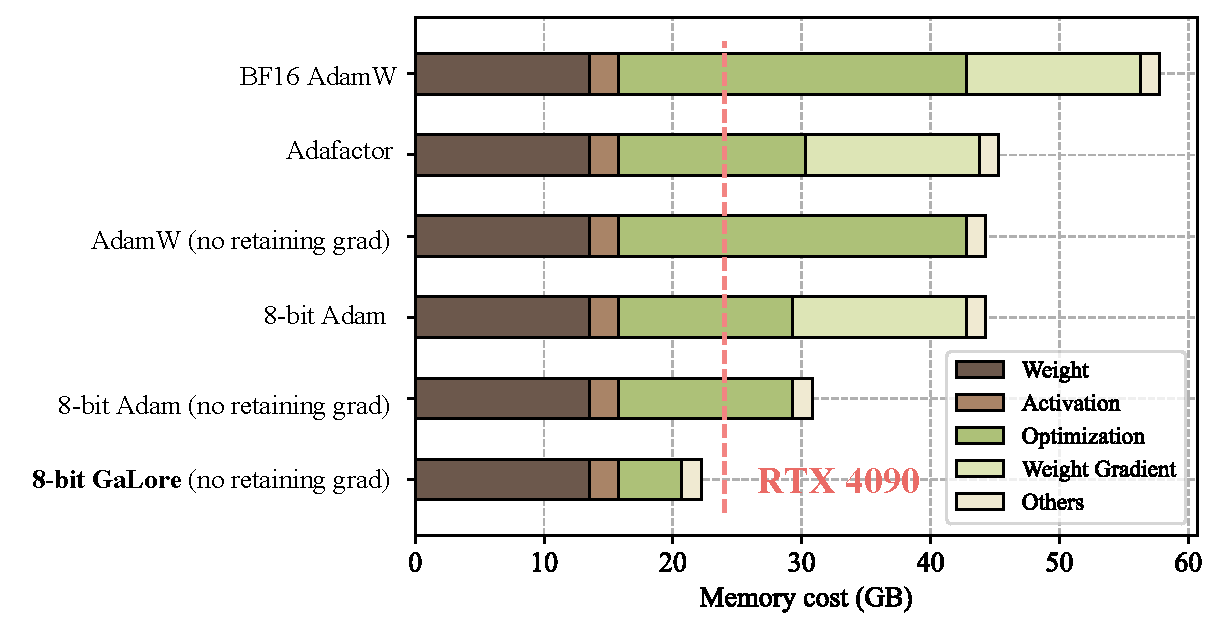
\includegraphics[width=1\columnwidth]{figures/files/memory_breakdown.pdf}
\vskip -0.11in
\caption{\small{Estimated memory consumption of pre-training a LLaMA 7B model with a token batch size of 256 on a single device, without activation checkpointing and memory offloading\protect\footnotemark[2]. Details refer to Section~\ref{sec:memory_measure}.}}
\label{fig:memory_breakdown} 
\vskip -0.15in
\end{figure}
\footnotetext[1]{The calculation is based on LLaMA architecture, BF16 numerical format, and maximum sequence length of 2048.}
\footnotetext[2]{In the figure, ``no retaining grad'' denotes the application of per-layer weight update to reduce memory consumption of storing weight gradient \citep{lvFullParameterFinetuning2023}.}
\SetAlFnt{\fontsize{8pt}{9pt}\selectfont}
\SetAlCapFnt{\fontsize{8pt}{9pt}\selectfont}
\begin{algorithm}[t]
    \SetAlgoLined
        \PyCode{for weight in model.parameters():} \\
        \Indp   %
            \PyCode{grad = weight.grad} \\ 
            \PyComment{original space -> compact space} \\
            \PyCode{lor\_grad = \textbf{project}(grad)} \\
            \PyComment{update by Adam, Adafactor, etc.} \\
            \PyCode{lor\_update = \textbf{update}(lor\_grad)} \\
            \PyComment{compact space -> original space} \\
            \PyCode{update = \textbf{project\_back}(lor\_update)} \\
            \PyCode{weight.data += update} \\
        \Indm %
    \caption{\fontsize{8pt}{9pt}\selectfont{\lowrank{}, PyTorch-like}}
    \label{alg:code_box}
\end{algorithm}


In order to implement the natural gradient transform, we need to compute the inverse of the Empirical Fisher Information Matrix and apply it to the gradient \(\mathbf{g_{k}}\). This can be done using the Woodbury Identity, which allows us to efficiently compute the inverse of a matrix of the form \(A + UBU^T\). The Woodbury Identity states that:

\[
(A + UBU^T)^{-1} = A^{-1} - A^{-1}U(B^{-1} + U^TA^{-1}U)^{-1}U^TA^{-1}
\]

Now if we choose

\begin{eqnarray}
    \mathbf{\hat{F}}_{k} &=& \lambda I + GG^{T} \\
    A &=& \lambda I \\
    U &=& G \\
    B &=& I \\
\end{eqnarray}

where \(G = [\operatorname{vec}(\mathbf{g_{k}}), \operatorname{vec}(\mathbf{g_{k-1}}),\ldots, \operatorname{vec}(\mathbf{g_{k-s}})]\) is the stacked gradient matrix over the past \(s \approx 20\) gradients and \(\lambda\) is a small constant for Tikhonov regularization, then the inverse of the empirical FIM applied to the gradient \(\mathbf{g_{k}}\) i.e. the natural gradient \(\mathbf{\tilde{g}}_{k} = \mathbf{\hat{F}}_{k}^{-1}\mathbf{g_{k}}\) can be computed as:

\begin{eqnarray}
    \mathbf{\tilde{g}}_{k} = \frac{1}{\lambda}\mathbf{g_{k}} - \frac{1}{\lambda^{2}}G\left(I + \frac{1}{\lambda}G^{T}G\right)^{-1}G^{T}\mathbf{g_{k}}
\end{eqnarray}

To compute the above formula efficiently, let \(S = I + \frac{1}{\lambda}G^{T}G \in \mathbb{R}^{s\times s}\) and \(y = G^T\mathbf{g_{k}}\). The idea is to use Cholesky decomposition to solve for \(z\) in
\begin{eqnarray}
S z = y
\end{eqnarray}
which can be done in \(\mathcal{O}(s^2)\) time. Then the natural gradient estimate can be computed using only matrix vector products, which is very memory efficient:
\begin{eqnarray}
    \mathbf{\tilde{g}}_{k} = \frac{1}{\lambda}\mathbf{g_{k}} - \frac{1}{\lambda^{2}}Gz
\end{eqnarray}

This natural gradient estimate can then be applied to the Adam optimizer \ref{eq:adam_update} and we update the model parameters, the same way as in GaLore. This allows us to efficiently incorporate second-order information into the optimization process, leading to faster convergence and better performance, especially in low-resource settings.